\chapter{Evaluation}\label{chapter:evaluation}

This chapter aims on presenting the concrete results that have been achieved using the respective approaches that were thoroughly explained in Chapter \ref{chapter:methodology} in order to provide an answer to the introduced research questions.

As illustrated by Figure \ref{fig:grafana-dashboard}, which gives an overview over the Grafana dashboard which was created and installed in order to visualize the energy-related data obtained from the individual deployments of the implemented Prometheus exporter, the edge systems employed in the experimental edge computing cluster were successfully enabled to poll the energy measurement data from the ESP32 powermeter and to propagate the data in the form of metrics to Prometheus. 

\begin{figure}[H]
    \centering
    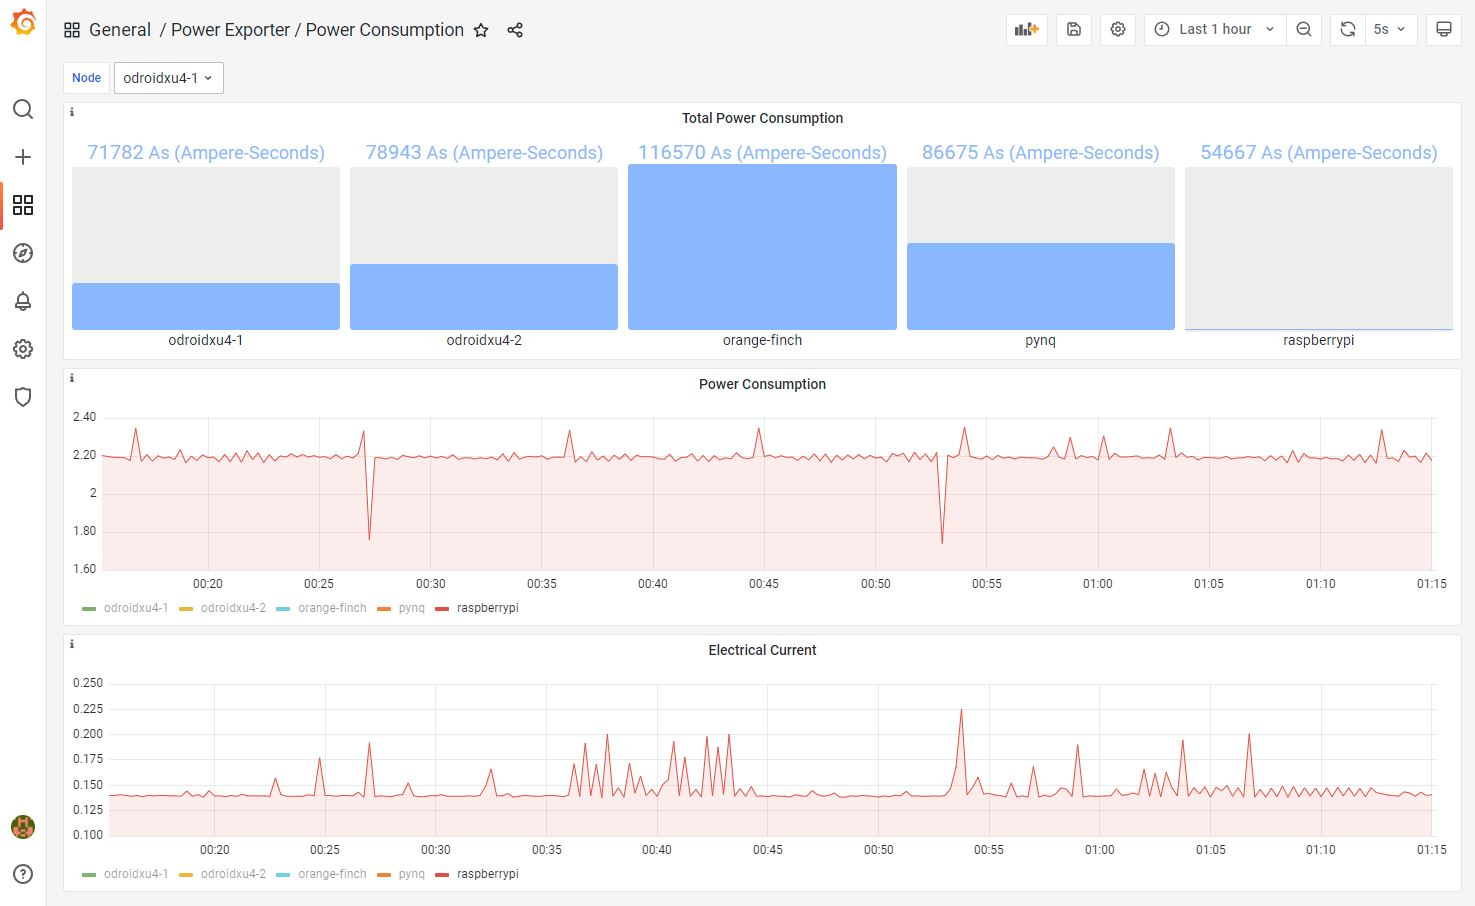
\includegraphics[width=\textwidth]{./figures/grafana-dashboard}
    \caption{Grafana Dashboard visualizing the energy-related data}
    \label{fig:grafana-dashboard}
\end{figure}

% \begin{figure}[H]
%     \centering
%     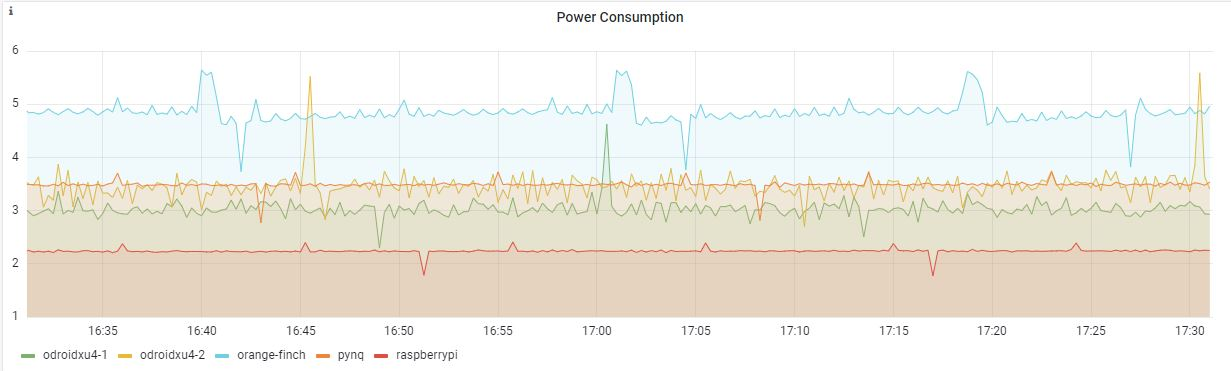
\includegraphics[width=\textwidth]{./figures/test}
%     \caption{Visualization of the current Energy Consumption per Edge-Device}
%     \label{fig:dashboard-power-consumption}
% \end{figure}

% \begin{figure}[H]
%     \centering
%     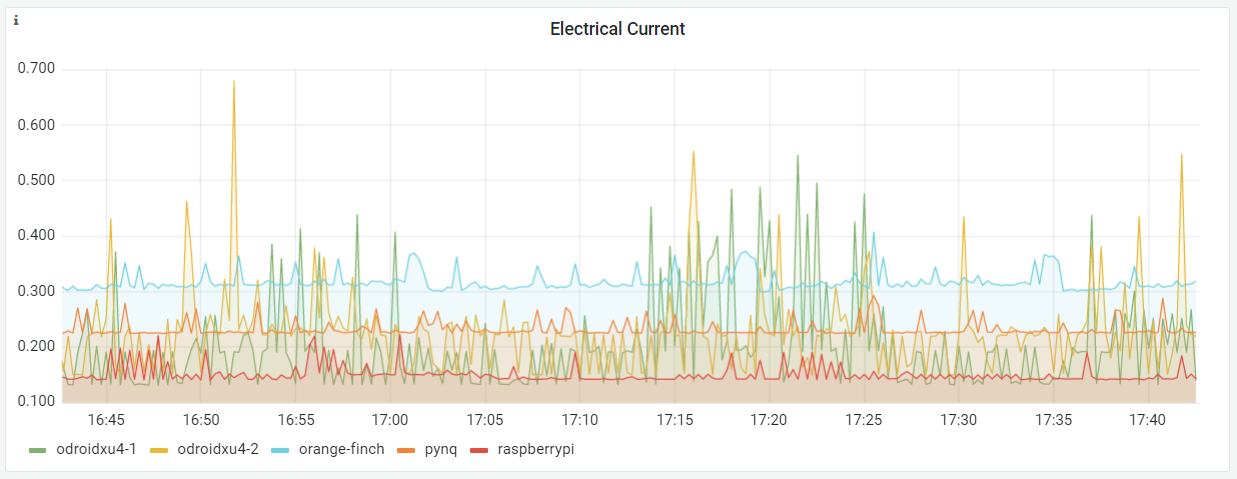
\includegraphics[width=\textwidth]{./figures/current}
%     \caption{Visualization of the Electrical Current per Edge-Device}
%     \label{fig:dashboard-current}
% \end{figure}

